\section{Parameter Identification: Physical Model}

\begin{frame}
	\frametitle{Discretization of the ODE}
	
	Discretize time interval:
	\begin{align*}
	  &[0,T] \rightarrow \left\{ 0=t_0, t_1, \dots, t_{m-1}, t_{m}=T 
\right\} \\
	\end{align*}
	
	Discretize state and control:
	\begin{align*}
	  &x_n = x(t_n) \\
   &u_n = u(t_n) \\
	\end{align*}
	
\end{frame}

\begin{frame}
	
	\frametitle{Discretization of the ODE}
	
% 	Solve ODE for every time step $h_n=t_{n+1}-t_n$ (Explicit Euler):
	Explicit Euler for every time step $h_n=t_{n+1}-t_n$:
	\begin{align*}
        &\Psi(x_n,u_n,p) = x_n + h_n f(x_n,u_n,p)  \\
	\end{align*}
	
	Discrete constraint:
	\begin{align*}
        &0 = x_{n+1} - \Psi(x_n,u_n,p) =: \Phi_n(x,u,p) \quad \forall n = 0,\ldots,m-1
	\end{align*}

	
\end{frame}

\begin{frame}
	\frametitle{Discretization of the ODE}
	
	\begin{figure}[bth]
	  \begin{center}
	    %left, bottom, right, top
	    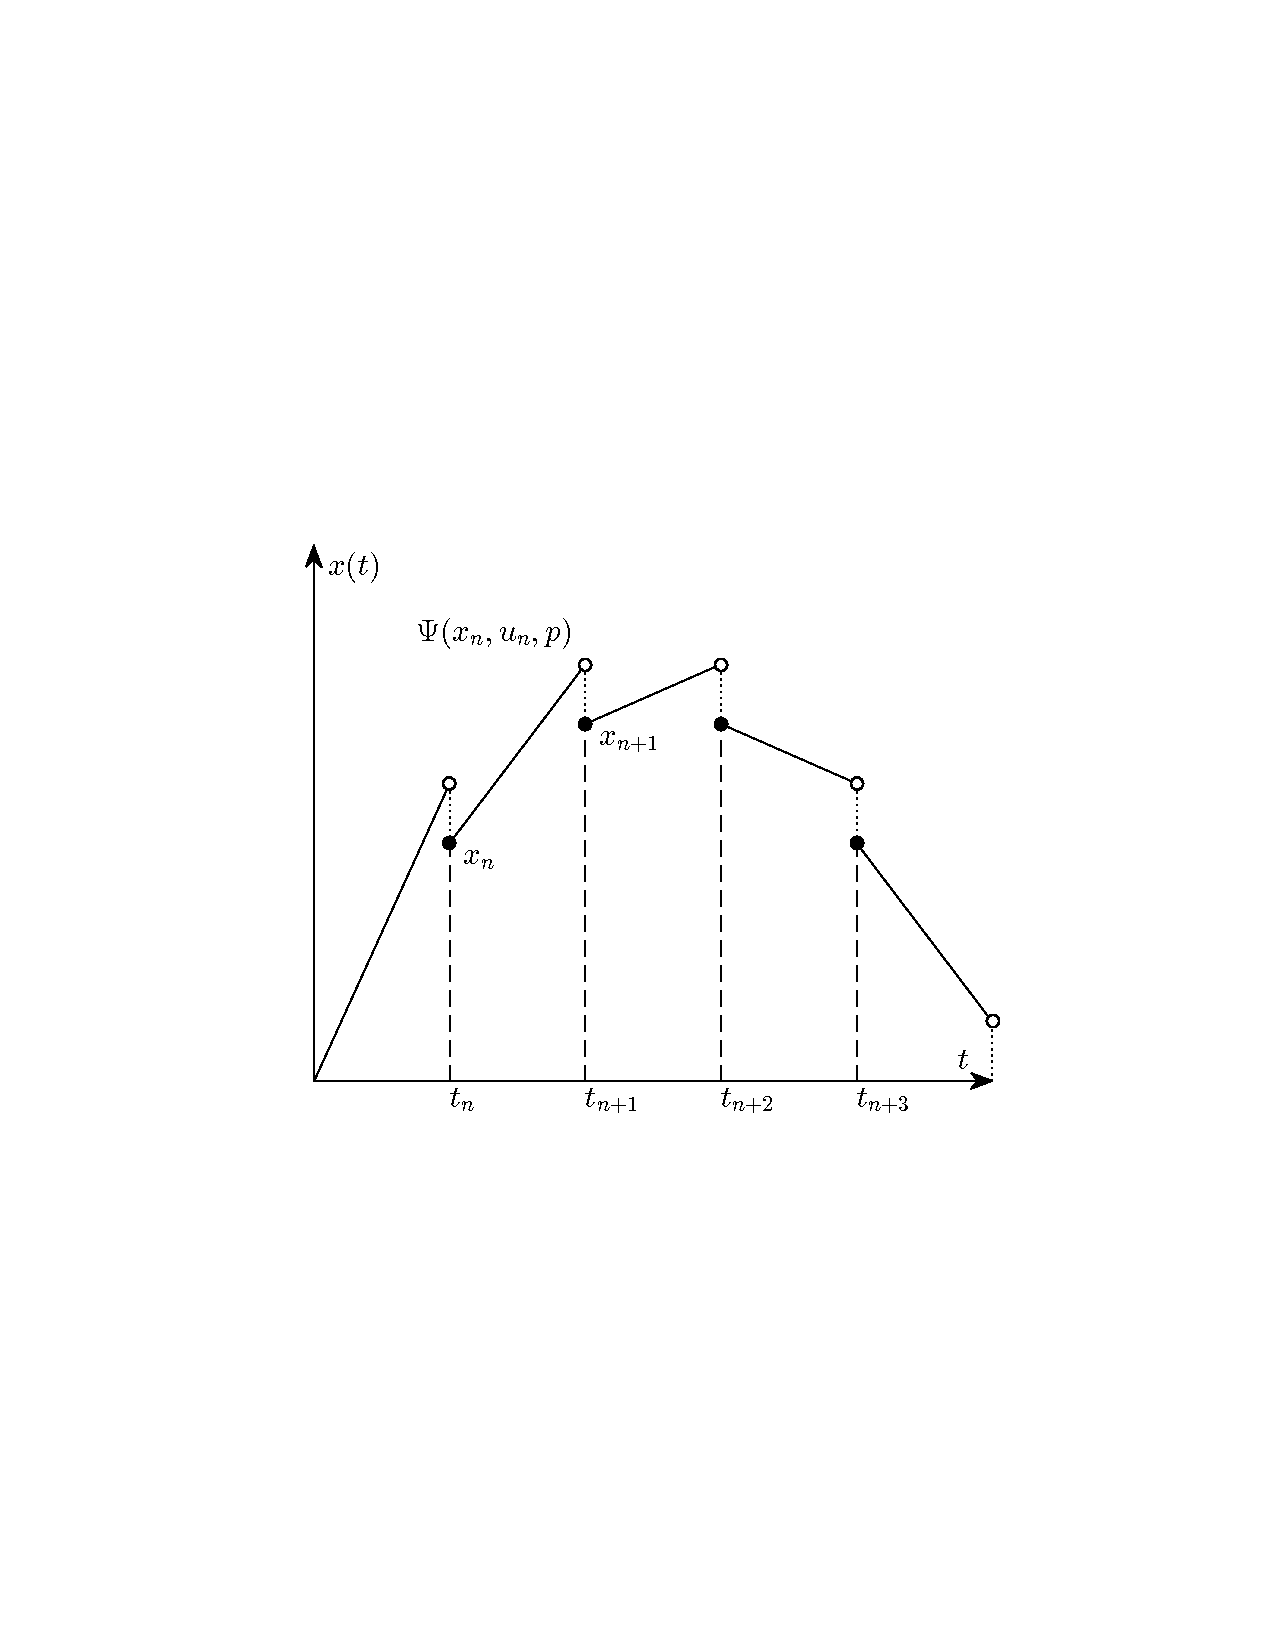
\includegraphics[trim=1cm 5cm 0cm 8cm, clip=true, width=\linewidth]{img/multShootPlot}
	  \end{center}
	\end{figure}
\end{frame}





\begin{frame}
    \frametitle{Problem Setting}
	\begin{columns}
	    
    
    \begin{column}{0.5\textwidth}
    Given:
    \begin{itemize}
        \item{control $\bar{u}$}
        \item{motion $\bar{x}$ related to $\bar{u}$ and $\bar{p}$}
    \end{itemize}

    Unknown:
    \begin{itemize}
        \item{parameters $\bar{p}$ of the excavator}
    \end{itemize}

    Output:
    \begin{itemize}
        \item{parameters $p$}
    \end{itemize}
    \end{column}
    
    \begin{column}{0.4\textwidth}

\includemedia[
  label      = DD,
  width      = 50mm,
  height     = 50mm,
  activate   = pageopen,
  addresource= videos/traj_x_ref3.mp4,
  flashvars={flv=videos/traj_x_ref3.mp4 & autoplay=1 & loop =1}
]{}{player_flv_maxi.swf}

\end{column}    
    
    
    
    \end{columns}
\end{frame}

\begin{frame}
    \frametitle{Problem Formulation}
    Natural approach: Optimal Control Problem
    \begin{align*}
        \min_{x,p} & & \frac{1}{2} \| \bar{x} - x \|^2 & & \\
        \operatorname{s.t.} & & \Phi(x,\bar{u},p) & = 0 & & \\
                            & & p & \geq 0 & & \\
    \end{align*}

    \begin{tabular}{ll}
        state & $ x = (s,\theta,\dot{s},\dot{\theta})^T $ \\
        parameters & $ p = (p_1,...,p_k)^T $ \\
        control & $ \bar{u} = (\tau_1,\tau_2)^T $ \\
        desired motion & $\bar{x}$ \\
    \end{tabular}
\end{frame}

%\begin{frame}
%    \frametitle{Problem Formulation}
%    \onslide<1->
%    Input:
%    \begin{itemize}
%        \item{control $\bar{u}$}
%        \item{desired motion $\bar{x}$ related to $\bar{u}$}
%    \end{itemize}
%
%    \onslide<2->
%    Output:
%    \begin{itemize}
%        \item{parameters $p$ of the excavator}
%        \item{x, but not of interest}
%    \end{itemize}
%
%    \onslide<3>
%    Idea:
%    \begin{itemize}
%        \item{get rid of variable $x$}
%        \item{set $x := \bar{x}$}
%        \item{solve a relaxed problem}
%    \end{itemize}
%\end{frame}

\begin{frame}
    \frametitle{Problem Formulation}

    \onslide<1->
    Original Problem
    \begin{align*}
        \min_{x,p} & & \frac{1}{2} \| \bar{x} - x \|^2 & & \\
        \operatorname{s.t.} & & \Phi(x,\bar{u},p) & = 0 & & \\
                            & & p & \geq 0 & & \\
    \end{align*}

    \onslide<2->
    Set $x \leftarrow \bar{x}$

    \onslide<3>
    Reinterpreted Problem
    \begin{align*}
        \min_{p}  & & \frac{1}{2} \| \Phi(\bar{x},\bar{u},p) \|^2 & & \\
        \operatorname{s.t.} & & p & \geq 0 & & \\
    \end{align*}
\end{frame}

\begin{frame}
    \begin{align*}
        \min_{p}  & & \frac{1}{2} \| \Phi(\bar{x},\bar{u},p) \|^2 & & \\
        \operatorname{s.t.} & & p & \geq 0 & & \\
    \end{align*}
    %\begin{align*}
    %    & \Phi_n(x,\bar{u},p) = x_{n+1} - \Psi(x_n,\bar{u}_n,p)   \quad \forall n = 0,\ldots,m-1 \\
    %\end{align*}
    \begin{itemize}
        \item{$\bar{x}$ solves ODE for $\bar{p}$}
        \item{$\Phi(\bar{x},\bar{u},\bar{p}) \rightarrow 0$ for discretization $m \rightarrow \infty$}
        \item{number of parameters fix}
    \end{itemize}
\end{frame}

\begin{frame}
    \frametitle{Comparison of the Approaches}

    \begin{columns}[t]
        \column{.5\linewidth}
            \begin{figure}
                \centering
                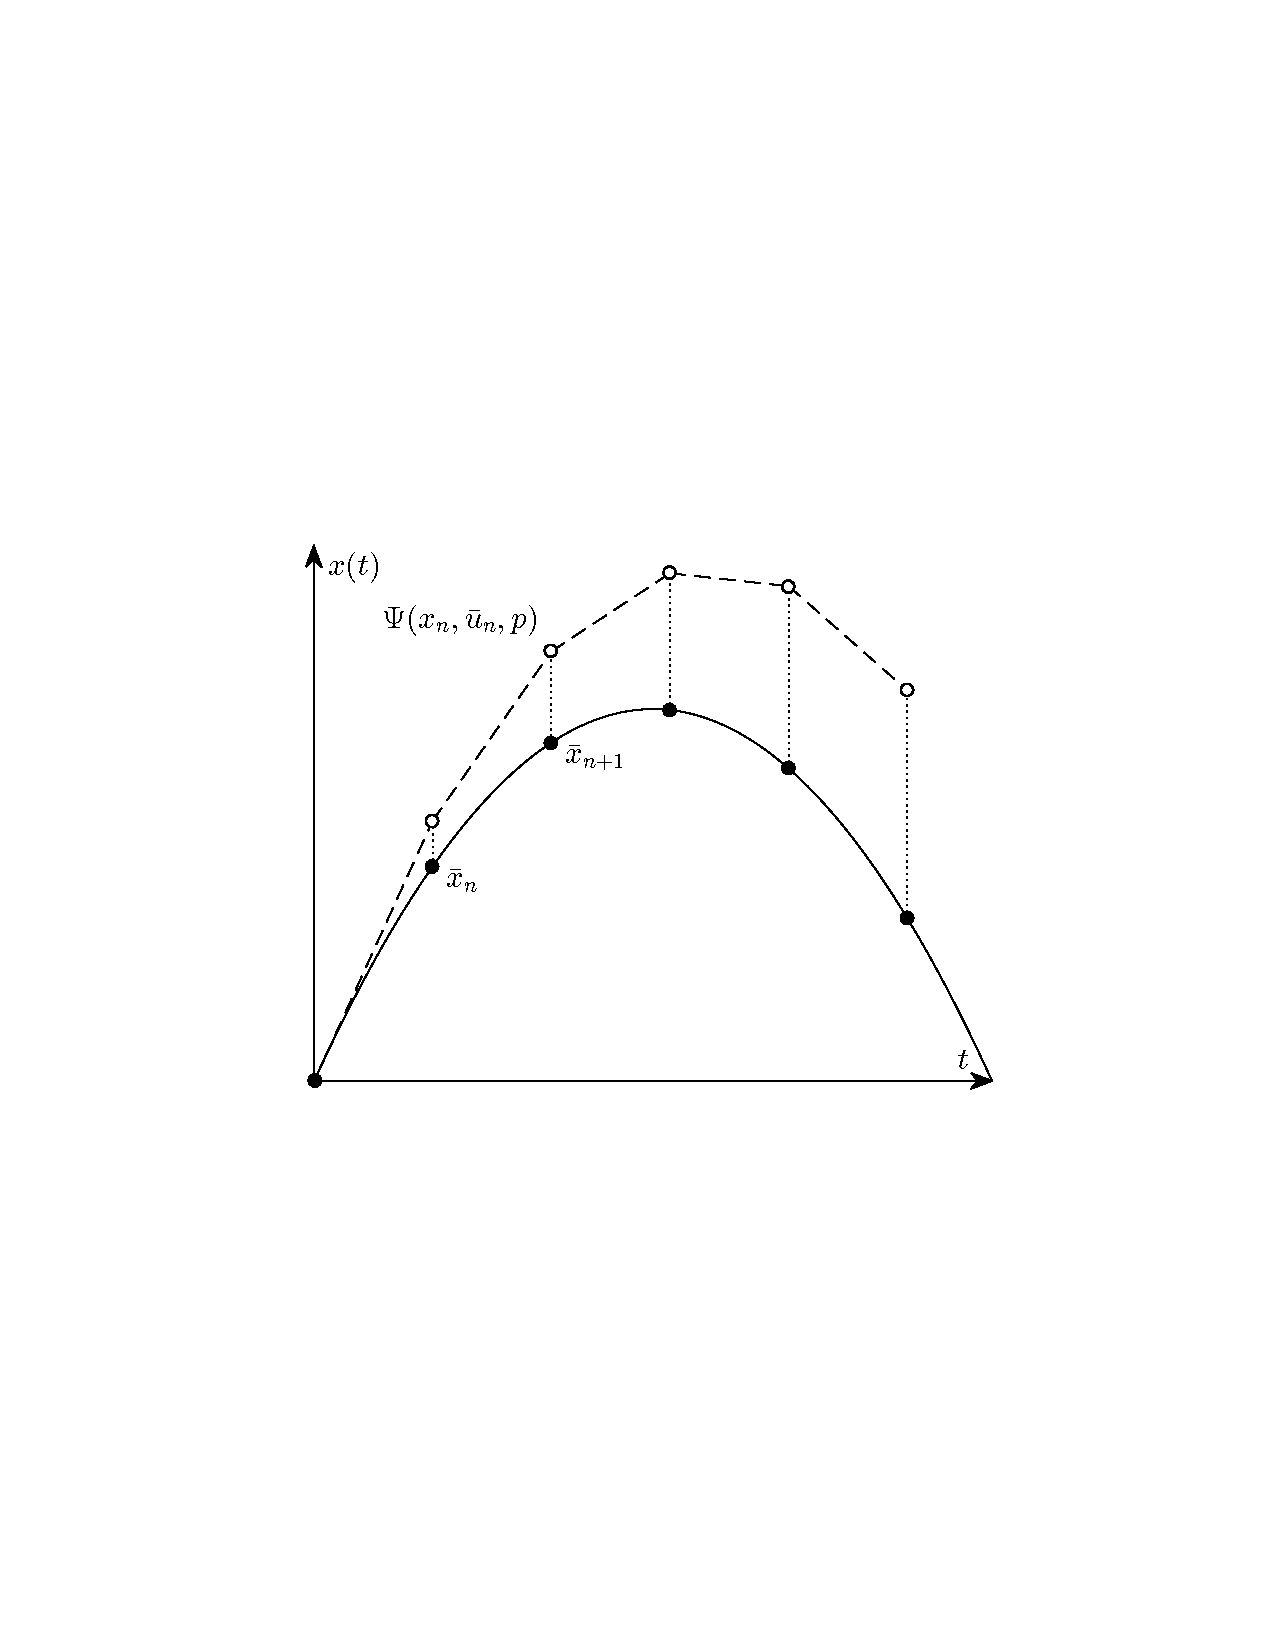
\includegraphics[trim=3cm 7cm 3cm 9cm, clip=true, width=\linewidth]{img/contExplEulerPlot}
            \end{figure}
        \column{.5\linewidth}
            \begin{figure}
                \centering
                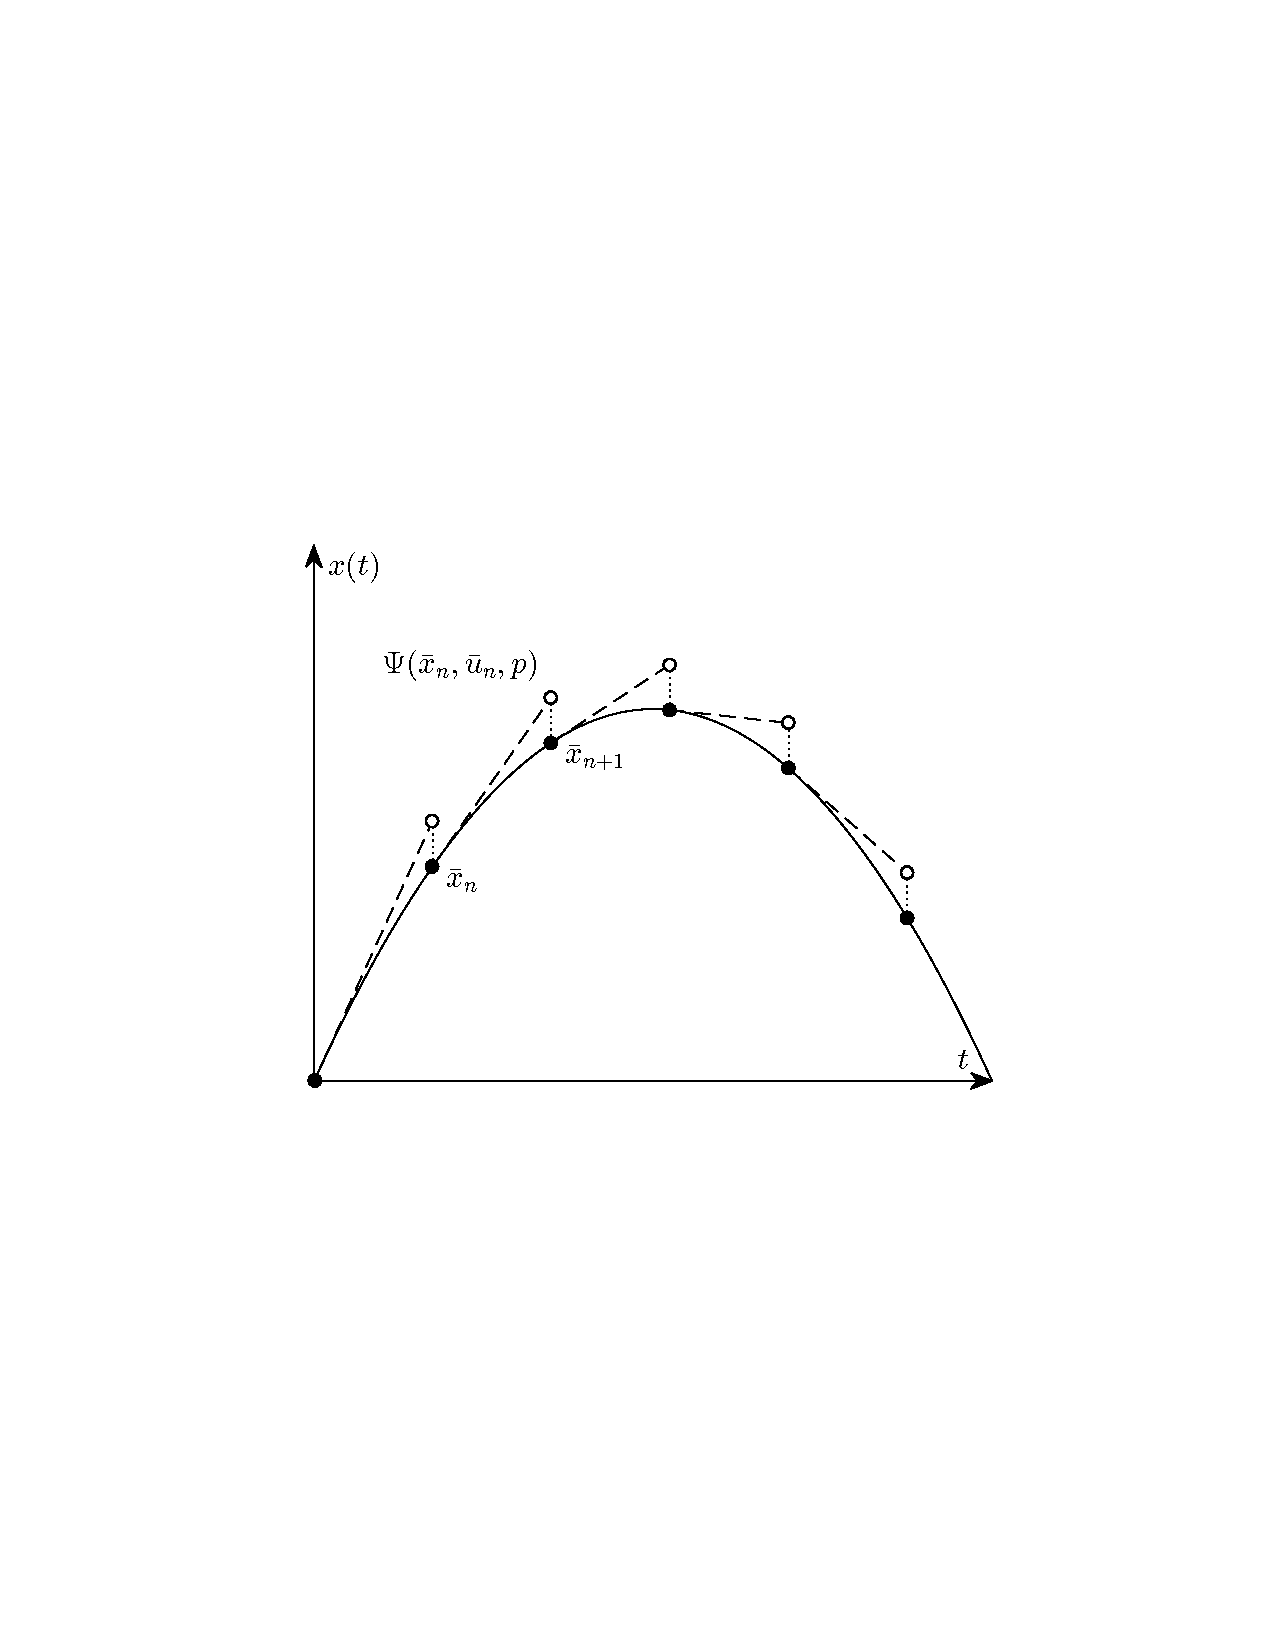
\includegraphics[trim=3cm 7cm 3cm 9cm, clip=true, width=\linewidth]{img/stepExplEulerPlot}
            \end{figure}
    \end{columns}
    \begin{center}
        continuous vs. stepwise Approximation
    \end{center}
\end{frame}

\begin{frame}
    \frametitle{Example Instance}
    \begin{itemize}
        \item{$[0,T] = [0,14s]$}
        \item{1500 time steps}
        \item{$p_0 \in [0.8  \bar{p}, 1.2  \bar{p}]$}
        \item{$x(p)$ solution of ODE for given $p$}
        \item{internally 5 trajectories in parallel}
    \end{itemize}

\end{frame}

\begin{frame}
    \frametitle{Results}
    \begin{columns}[t]
        \column{.5\linewidth}
            \begin{figure}
                \centering
                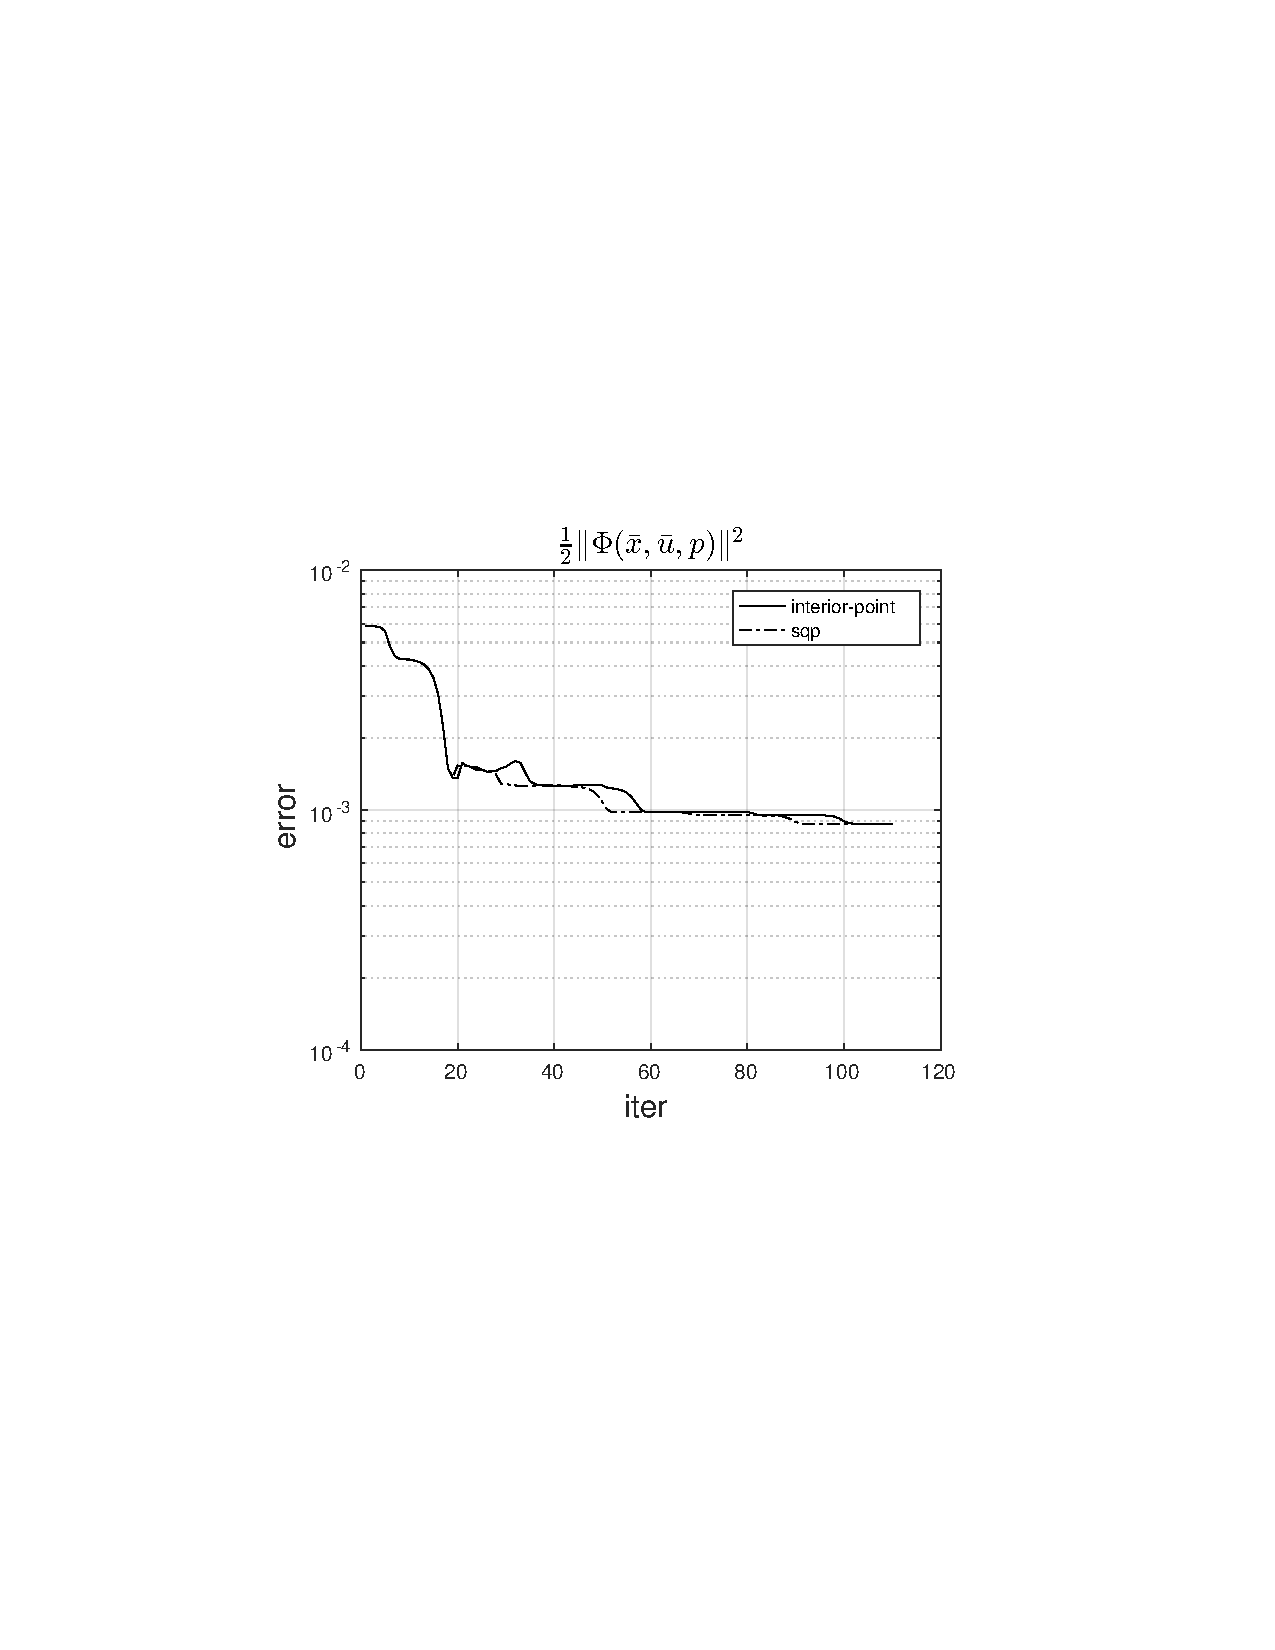
\includegraphics[trim=4cm 9cm 4cm 8.5cm, clip=true, width=\linewidth]{img/convPlotPhi}
            \end{figure}
        \column{.5\linewidth}
            \begin{figure}
                \centering
                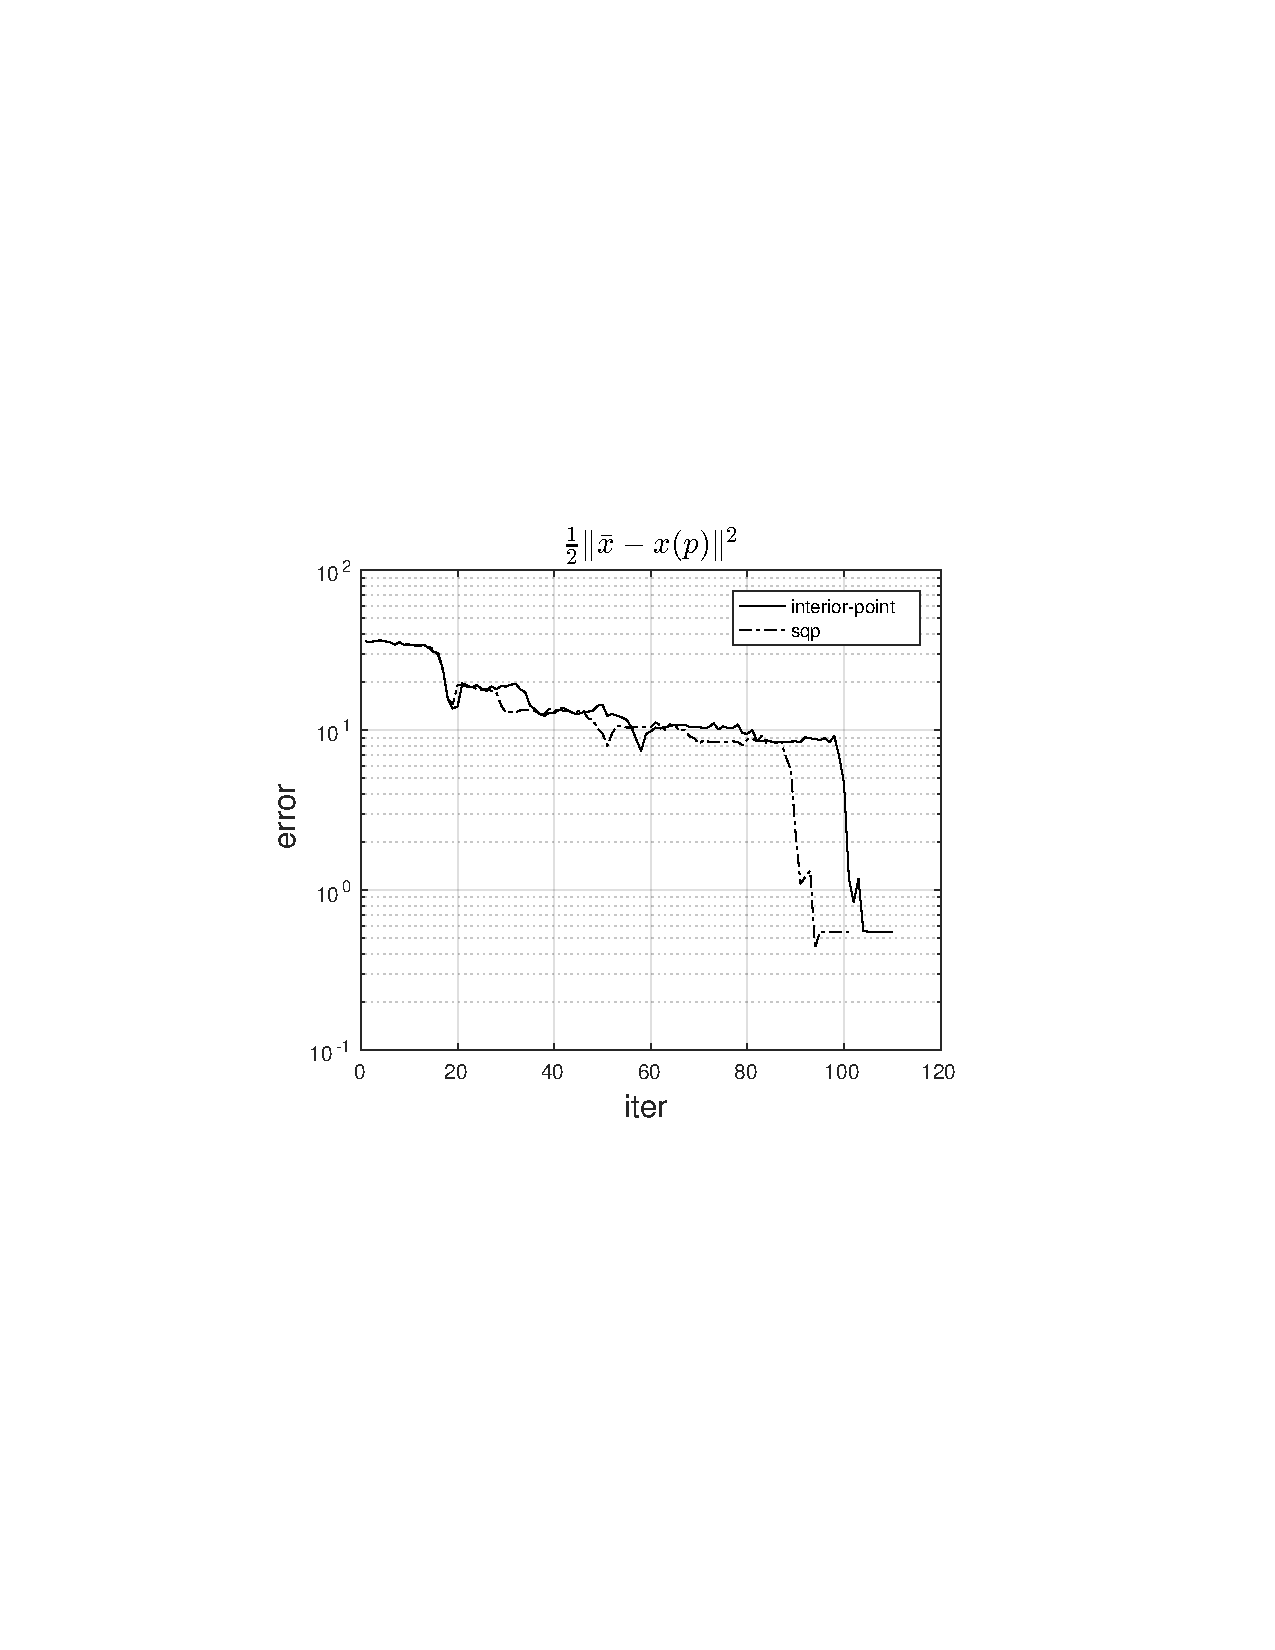
\includegraphics[trim=4cm 9cm 4cm 8.5cm, clip=true, width=\linewidth]{img/convPlotX}
            \end{figure}
    \end{columns}
\end{frame}

\begin{frame}
    \frametitle{Results}

    \begin{columns}[t]
        \column{.5\linewidth}
            \begin{figure}
                \centering
                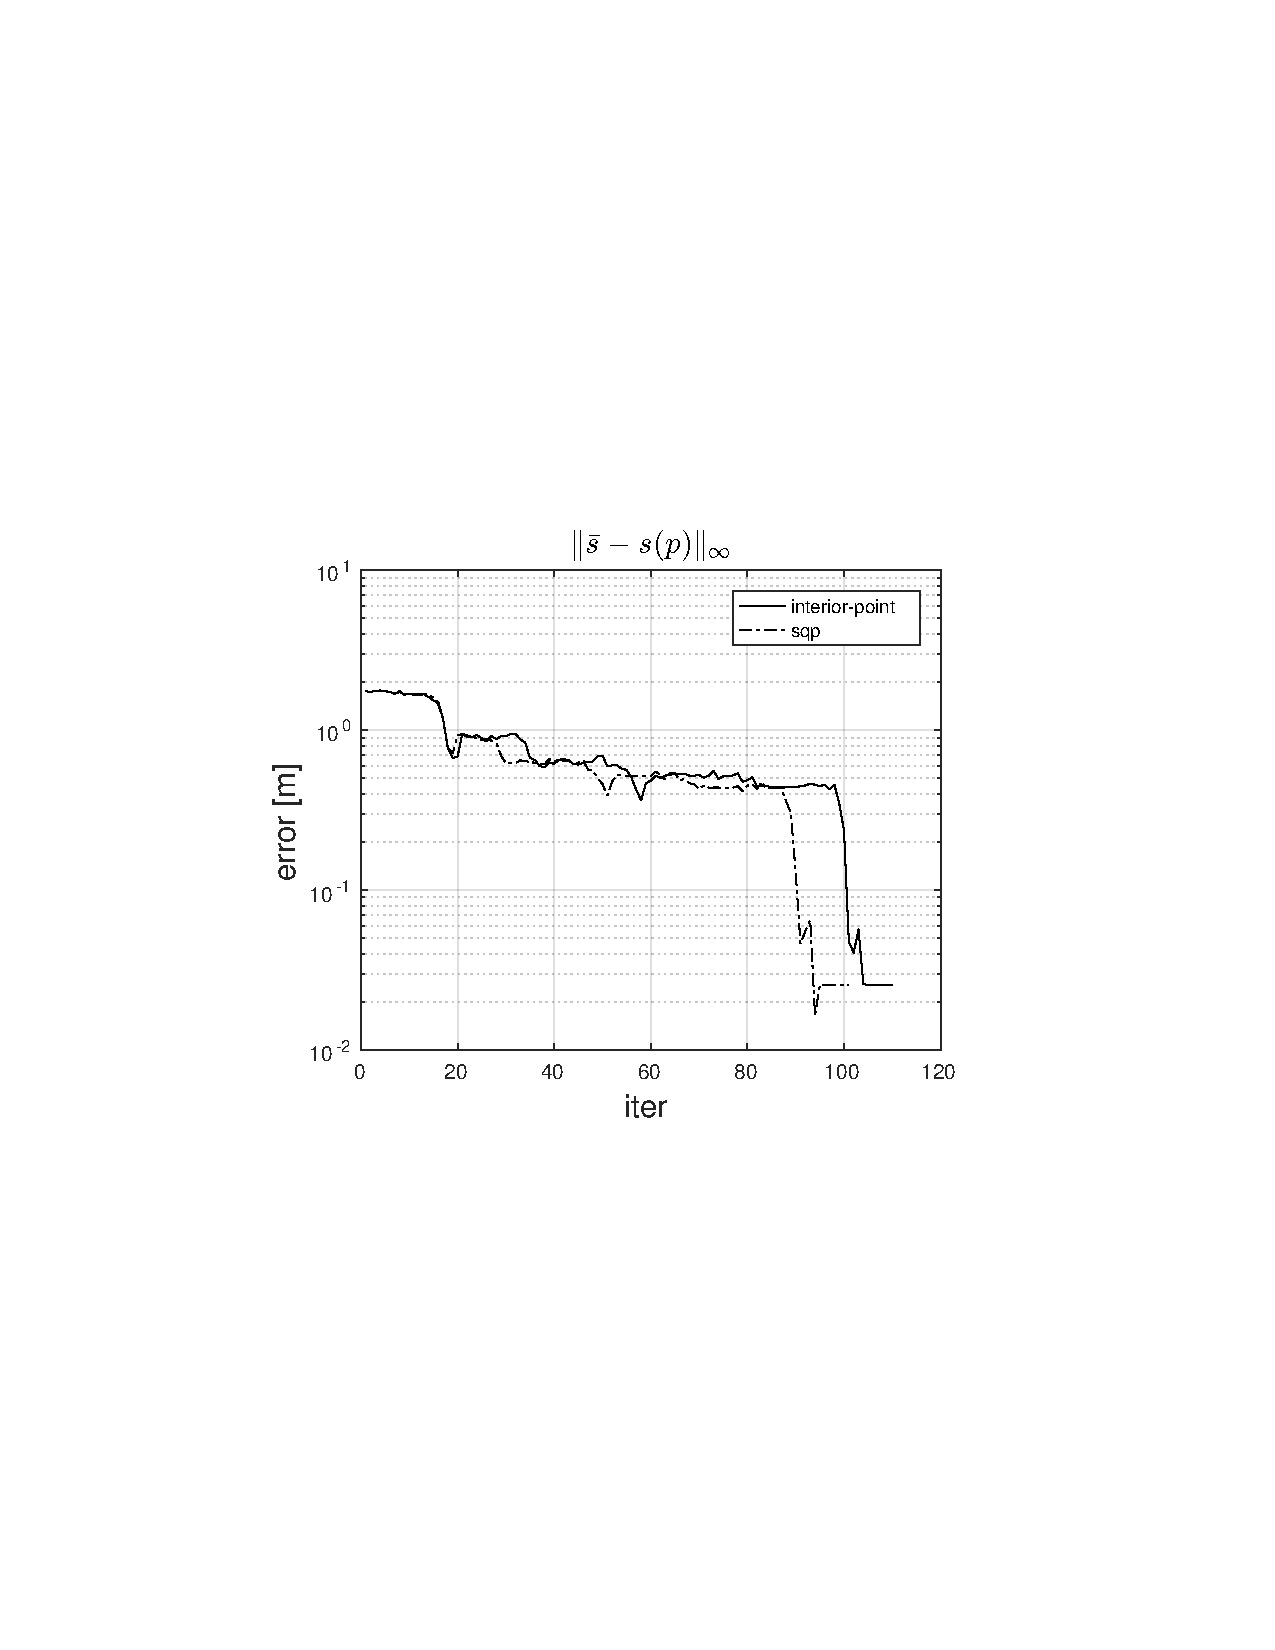
\includegraphics[trim=4cm 9cm 4cm 8.5cm, clip=true, width=\linewidth]{img/convPlotS}
            \end{figure}
        \column{.5\linewidth}
            \begin{figure}
                \centering
                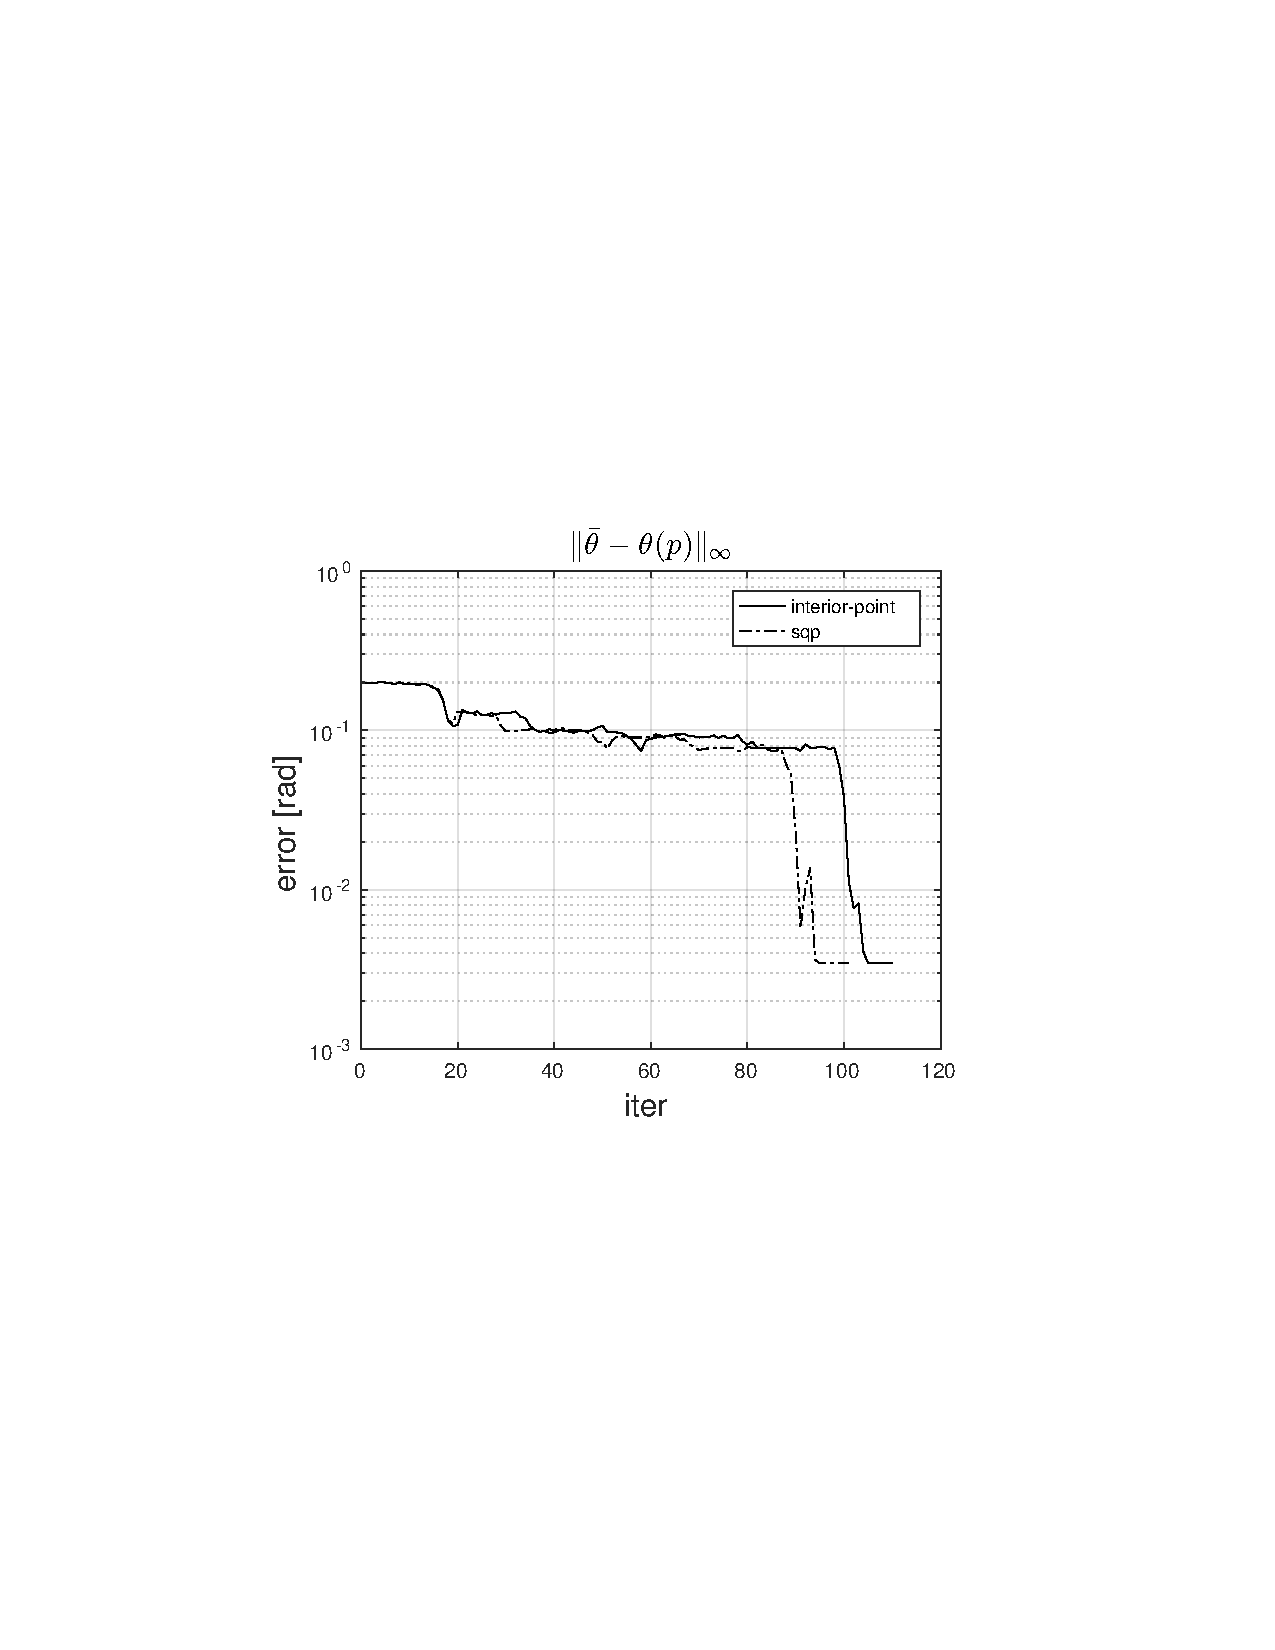
\includegraphics[trim=4cm 9cm 4cm 8.5cm, clip=true, width=\linewidth]{img/convPlotT}
            \end{figure}
    \end{columns}

    \begin{center}
        Exact up to $3\text{cm}$
    \end{center}
\end{frame}

\begin{frame}
    \frametitle{Results}
    \begin{columns}[t]
        \column{.5\linewidth}
            \begin{figure}
                \centering
                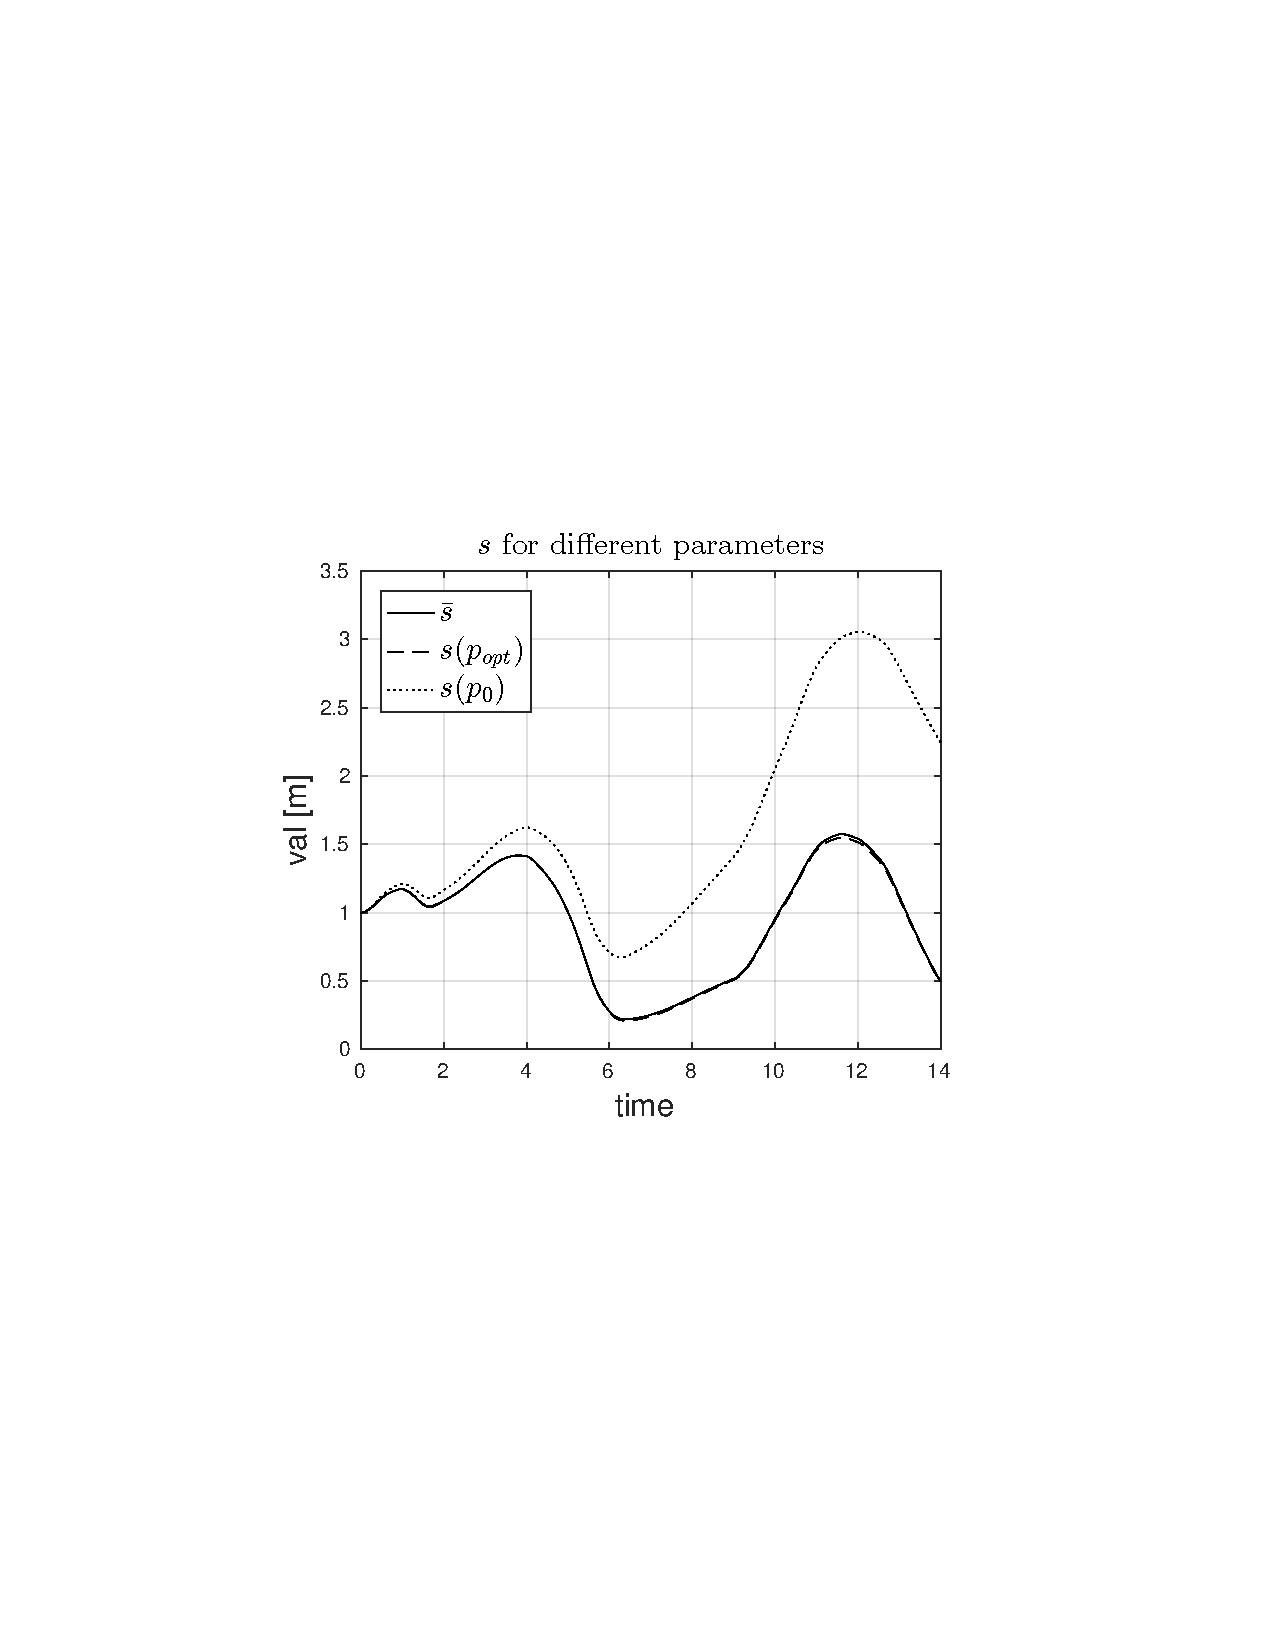
\includegraphics[trim=4cm 9cm 4cm 8.5cm, clip=true, width=\linewidth]{img/convPlotTrajS}
            \end{figure}
        \column{.5\linewidth}
            \begin{figure}
                \centering
                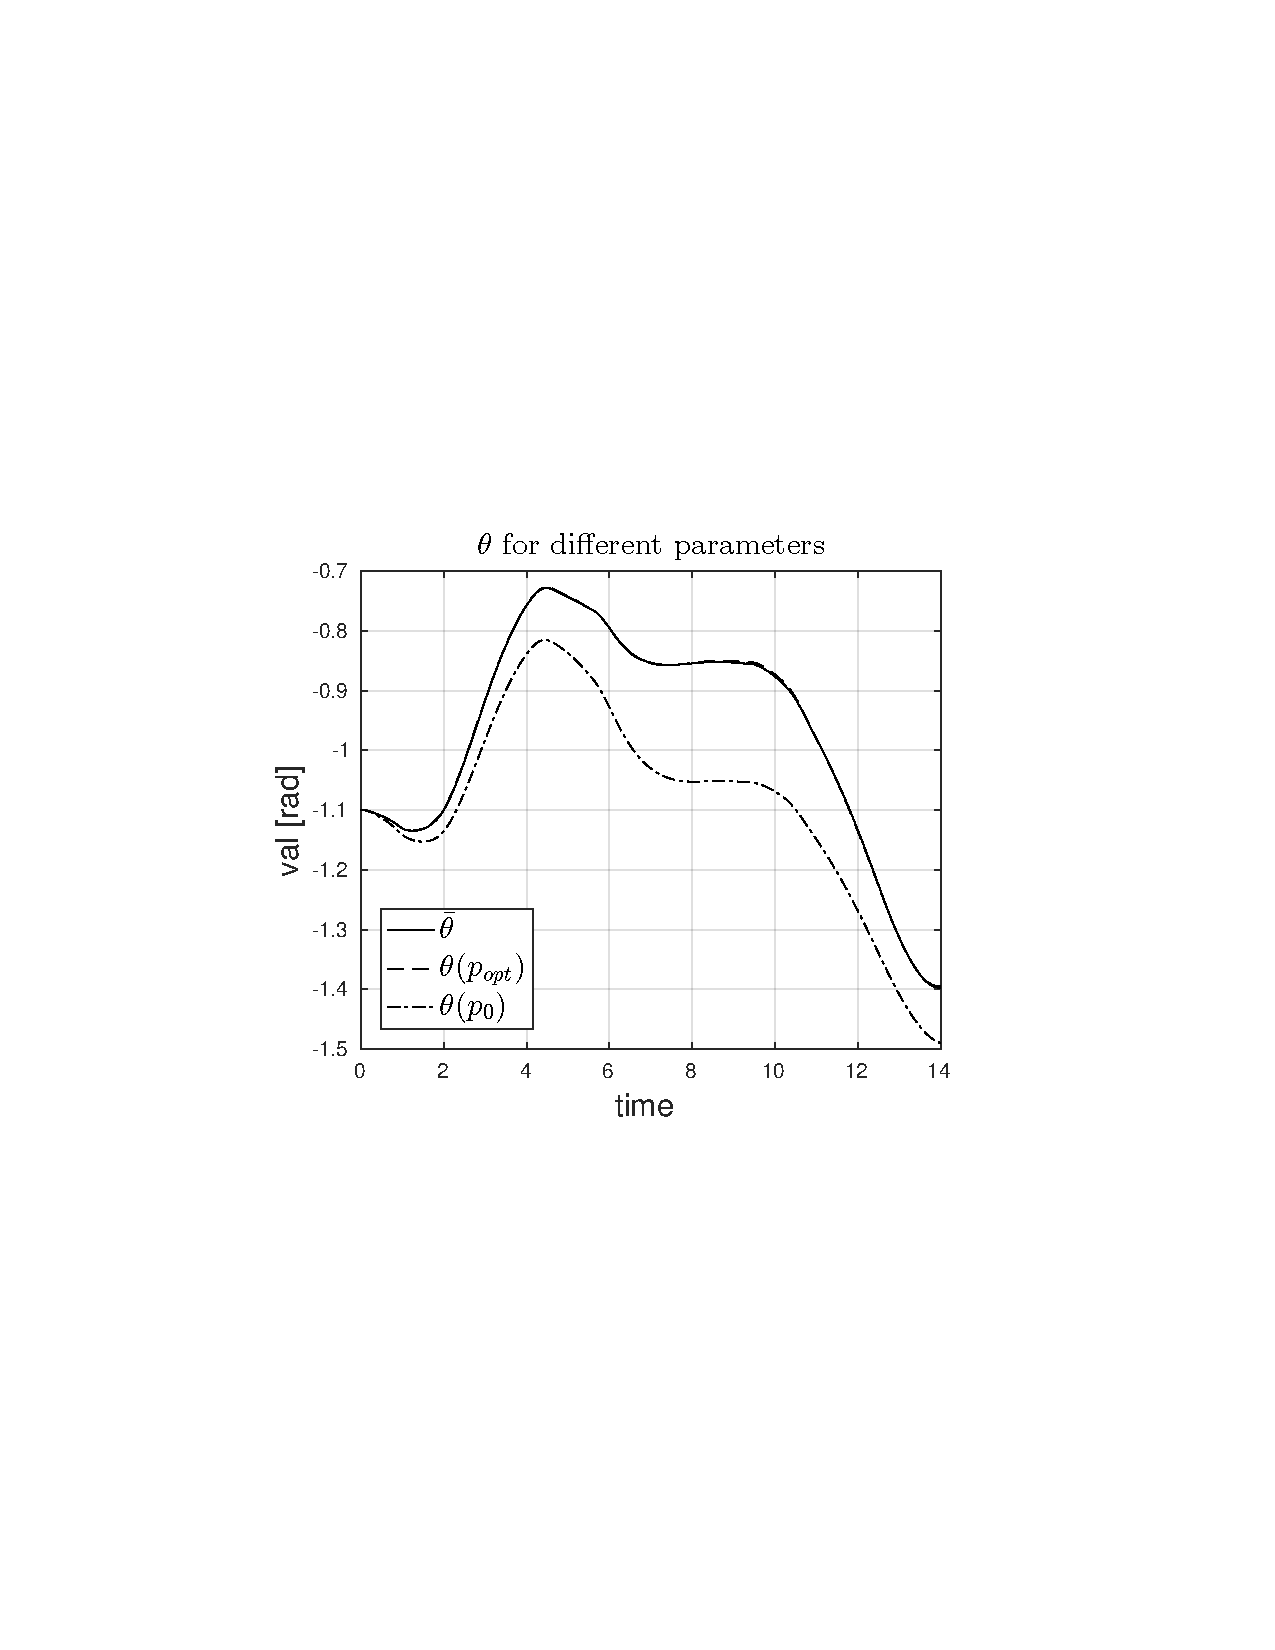
\includegraphics[trim=4cm 9cm 4cm 8.5cm, clip=true, width=\linewidth]{img/convPlotTrajT}
            \end{figure}
    \end{columns}
\end{frame}
